\documentclass[11pt,a4paper]{book}
\usepackage[brazilian]{babel}
\usepackage[utf8]{inputenc}
\usepackage[T1]{fontenc}
\usepackage[inline]{enumitem}
\usepackage{xcolor}
\usepackage{listings}
\usepackage{graphicx}
\usepackage{multicol}
\usepackage{amsmath}

\definecolor{mGreen}{rgb}{0,0.6,0}
\definecolor{mGray}{rgb}{0.5,0.5,0.5}
\definecolor{mPurple}{rgb}{0.58,0,0.82}
\definecolor{backgroundColour}{rgb}{0.95,0.95,0.92}

\lstdefinestyle{CStyle}{
    backgroundcolor=\color{backgroundColour},   
    commentstyle=\color{mGreen},
    keywordstyle=\textbf{\color{black}},
    numberstyle=\tiny\color{mGray},
    stringstyle=\color{mPurple},
    basicstyle=\footnotesize,
    breakatwhitespace=false,         
    breaklines=true,                 
    captionpos=b,                    
    keepspaces=true,                 
    numbers=left,                    
    numbersep=5pt,                  
    showspaces=false,                
    showstringspaces=false,
    showtabs=false,                  
    tabsize=2,
    frame=single,
    escapeinside={(*}{*)},
    language=C
}

\makeatletter
% This command ignores the optional argument for itemize and enumerate lists
\newcommand{\inlineitem}[1][]{%
\ifnum\enit@type=\tw@
    {\descriptionlabel{#1}}
  \hspace{\labelsep}
\else
  \ifnum\enit@type=\z@
       \refstepcounter{\@listctr}\fi
    \quad\@itemlabel\hspace{\labelsep}
\fi}
\makeatother

\newcommand{\onestaritem}{\refstepcounter{enumi}\item[$*$\theenumi.]}
\newcommand{\twostaritem}{\refstepcounter{enumi}\item[$**$\theenumi.]}

\title{Lista 2: Fundamentos Estatísticos para Ciência dos Dados}
\author{Ricardo Pagoto Marinho}

\begin{document}
\maketitle
	\begin{enumerate}
		\item
			\begin{lstlisting}
gMean=function(x){
	L <- length(x)
	p <- prod(x)
	if(any(x<0))
		warning("Valor(es) negativo(s) no vetor")
	return(p^(1/L))
}
			\end{lstlisting}
		\item
			\begin{itemize}
				\item
					$
					x<-apply(data,2,gMean)
					$
				\item
					$
					stdDev<-apply(data,2,sd)					
					$
				\item
					$
					s<-apply(data,1,sum)
					$
				\item
					$
					which(data\$X.1>3 \& data\$X.20<3)
					$\\
					Apareceram 102 linhas
				\item
					$
					colnames(data)<-paste("Var",1:25,sep="")
					$
			\end{itemize}
		\item
			\begin{itemize}
				\item
					$
					boxplot(iris\$Sepal.Length,iris\$Sepal.Width,iris\$Petal.Length,iris\$Petal.Width,iris\$Species)
					$
				\item
					\begin{lstlisting}
par(mfrow=c(2,2))
boxplot(Sepal.Length ~ Species,data = iris)
boxplot(Sepal.Width ~ Species,data = iris)
boxplot(Petal.Length ~ Species,data = iris)
boxplot(Petal.Width ~ Species,data = iris
					\end{lstlisting}
				\item
					\begin{lstlisting}
par(mfrow=c(2,3))
hist(iris\$Sepal.Length)
hist(iris\$Sepal.Width)
hist(iris\$Petal.Length)
hist(iris\$Petal.Wis)
hist(iris\$Petal.Width)
					\end{lstlisting}
			\end{itemize}
		\item
			\begin{itemize}
				\item
					\begin{figure}[b]
					\centering
					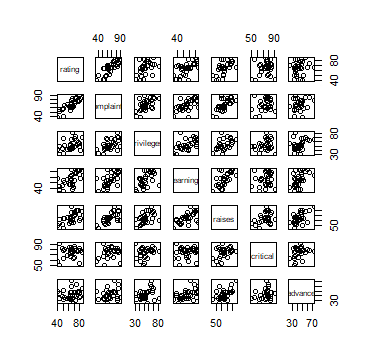
\includegraphics[height=5cm]{Rplot.png}
					\caption{plot(attitude)}
					\end{figure}
				\item
					\begin{lstlisting}
m<-apply(attitude,2,mean)
m
    rating complaints privileges   learning     raises   critical    advance 
  64.63333   66.60000   53.13333   56.36667   64.63333   74.76667   42.93333 
					\end{lstlisting}
				\item
					\begin{lstlisting}
cut(attitude$complaints,breaks = c(0,60,80,100), labels = c("bad","okay","good"))
 [1] bad  okay okay okay okay bad  okay okay good okay bad  bad  okay good okay good good bad  okay bad  bad  okay
[23] okay bad  bad  okay okay bad  good good
Levels: bad okay good
					\end{lstlisting}
				\item
					\begin{lstlisting}
x<-cut(attitude$complaints,breaks = c(0,60,80,100), labels = c("bad","okay","good"))
boxplot(rating ~ x,data=attitude)
					\end{lstlisting}
					\begin{figure}[b]
					\centering
					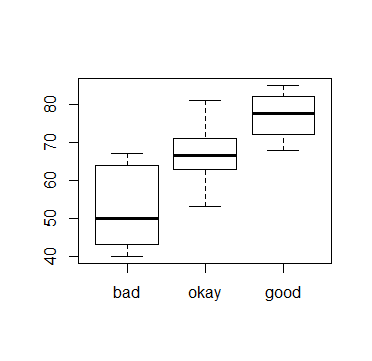
\includegraphics[height=5cm]{Rplot01.png}
					\caption{rating x complaints}
					\end{figure}
			\end{itemize}
	\end{enumerate}
\end{document}